\documentclass{article}
\usepackage{tikz}
\usetikzlibrary{datavisualization}
\title{CSL 603 - Machine Learning\\Lab 1\\Decision Trees and Forests}
\author{Aditya Gupta\\2015csb1003}
\begin{document}
\maketitle
\section*{Decision Tree (Experiment 2)}
A decision tree was learnt using 1000 reviews from the train set and tested on 1000 reviews from the test set. The learned tree showed the following statistics:
\subsection{Effect of Early Stopping}
The tree propagation was stopped when a critical height was reached and various properties of the tree such as total terminal nodes (leaf nodes) and the accuracy was noted. The following results were obtained:

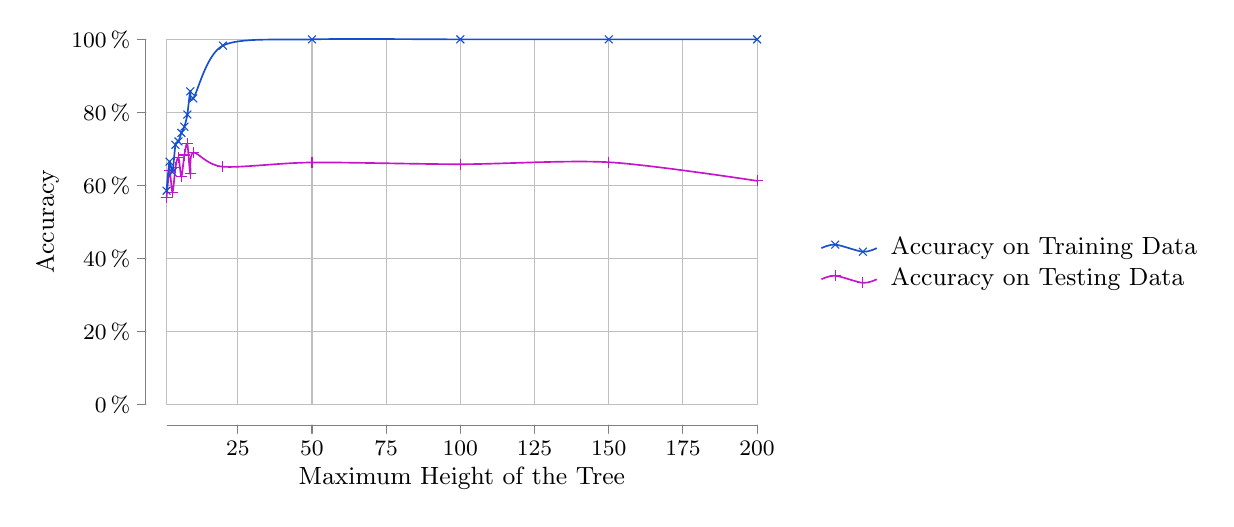
\begin{tikzpicture}[scale=1.5]
\datavisualization [scientific axes=clean,
	x axis={grid, label={Maximum Height of the Tree}},
	y axis={grid, label={Accuracy}, ticks ={tick unit=\%}, min value=0, max value=100},
	visualize as smooth line/.list={trainacc, testacc},
	style sheet=vary hue,
	style sheet=cross marks,
	trainacc={label in legend={text=Accuracy on Training Data}},
	testacc={label in legend={text=Accuracy on Testing Data}}]
data [set=trainacc] {
	x, y
	1, 58.534
	2, 66.499
	3, 63.645
	4, 71.111
	5, 72.032
	6, 74.361
	7, 76.0692
	8, 79.405
	9, 85.757
	10, 83.819
	20, 98.300
	50, 100.0
	100, 100.0
	150, 100.0
	200, 100.0
}
data [set=testacc] {
	x, y
	1, 56.592
	2, 64.012
	3, 58.074
	4, 64.878
	5, 67.679
	6, 62.449
	7, 68.3049
	8, 71.342
	9, 63.242
	10, 68.965
	20, 65.102
	50, 66.266
	100, 65.789
	150, 66.332
	200, 61.226
};
\end{tikzpicture}

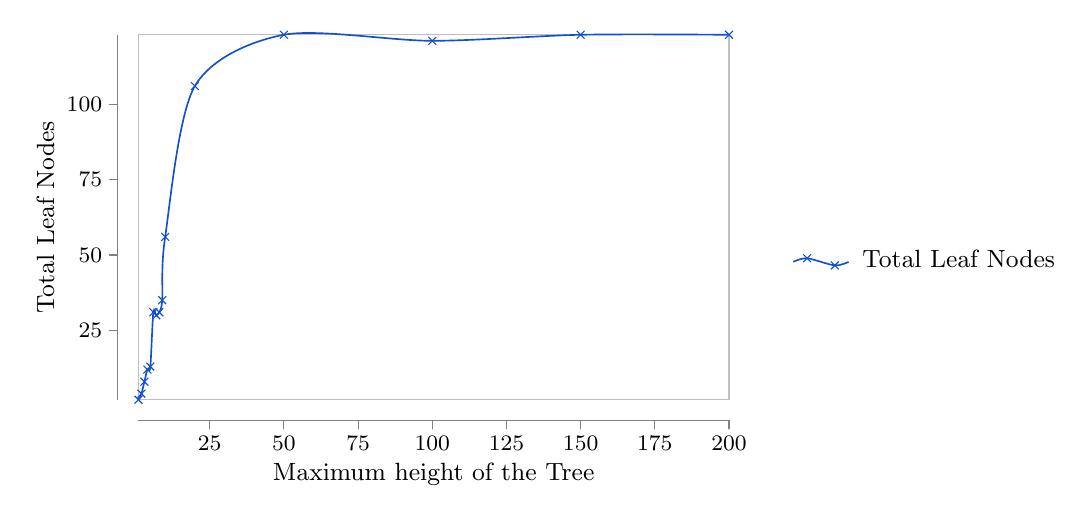
\begin{tikzpicture}[scale=1.5]
\datavisualization [scientific axes=clean,
	visualize as smooth line/.list={leaf},
	style sheet=vary hue,
	style sheet=cross marks,
	x axis={label={Maximum height of the Tree}},
	y axis={label={Total Leaf Nodes}},
	leaf={label in legend={text=Total Leaf Nodes}}]
data [set=leaf]{
x, y
1, 2
2, 4
3, 8
4, 12
5, 13
6,  31
7, 30
8, 31
9, 35
10, 56
20, 106
50, 123
100, 121
150, 123 
200, 123
};
\end{tikzpicture}
\section*{Noise (Experiment 3)}
The Noise was changed and the following results were obtained:

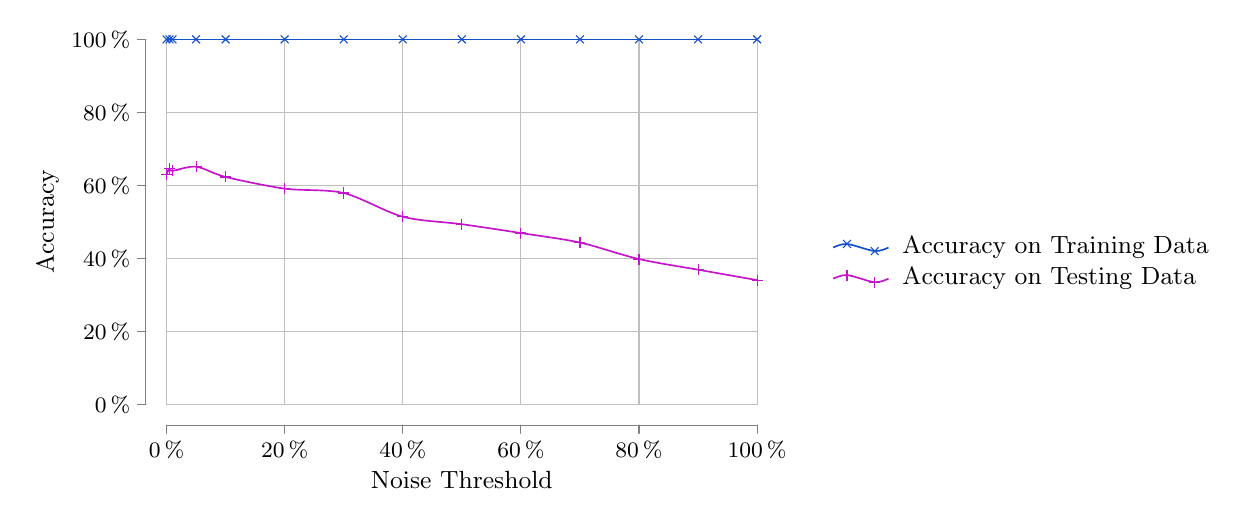
\begin{tikzpicture}[scale=1.5]
\datavisualization [scientific axes=clean,
	x axis={grid, label={Noise Threshold}, ticks={tick unit=\%}},
	y axis={grid, label={Accuracy}, ticks ={tick unit=\%}, min value=0, max value=100},
	visualize as smooth line/.list={trainacc, testacc},
	style sheet=vary hue,
	style sheet=cross marks,
	trainacc={label in legend={text=Accuracy on Training Data}},
	testacc={label in legend={text=Accuracy on Testing Data}}]
data [set=trainacc] {
	x, y
	0, 100.0
	0.5, 100.0
	1, 100.0
	5, 100.0
	10, 100.0
	20, 100.0
	30, 100.0
	40, 100.0
	50, 100.0
	60, 100.0
	70, 100.0
	80, 100.0
	90, 100.0
	100, 100.0
}
data [set=testacc] {
	x, y
	0, 63.039
	0.5, 64.604
	1, 63.975
	5, 65.111
	10, 62.298
	20, 59.1
	30, 57.894
	40, 51.398
	50, 49.349
	60, 46.928
	70, 44.321
	80, 39.796
	90, 36.884
	100, 34.036
};
\end{tikzpicture}

\section*{Pruning (Experiment 4)}
Lorem Ipsum bla bla bla
\section*{Decision Forests (Experiment 5)}
Lorem Ipsum bla bla bla
\end{document}